\chapter{Di-$b$-jet Search: Limit Setting}
\label{sec:lim}

In Chapter~\ref{sec:bkg} it was shown that there was no evidence of signal in the dijet spectra considered.
Specifically, what was found was that the probability of obtaining a data-set with an excess similar to the one observed
under the assumption that there is new physics was above a certain threshold.
This lead to the conclusion that there is no evidence of BSM physics in the di-$b$-jet spectra.

However, it is also useful to further quantify this observation by asking the question
`if a new physics model was true would it have be observed in the di-$b$-jet spectrum?'
If there are physics models that we are confident that we would have seen, then we can exclude them.
This process is known as limit setting.

In this Chapter,
Section~\ref{sec:lim-strat} will describe the limit setting strategy used,
Section~\ref{sec:lim-syst} will list the systematics considered
and Section~\ref{sec:lim-summer} and Section~\ref{sec:lim-full}
shows the results for the various data-sets considered.

\section{Bayesian Limits}
\label{sec:lim-strat}

For Bayesian limit setting, we invert the hypothesis test set out in the search phase;
instead let us assume as the null hypothesis that there is a new physics resonance
which produces $\mu$ di-$b$-jet events per~\ifb~in some known shape in~\mjj.
This signal is produced in addition to the QCD background,
which has been modelled by the background fit from the previous chapter.
This signal plus background model can be denoted with the hypothesis $H_\mu$.

Now let us consider this hypothesis in the context of the data,
which in this case is one of our di-$b$-spectra, and is denoted by $D$.
Let's say that in each~\mjj~bin, the model predicts
$s_i$ signal events, $b_i$ background events and $n_i$ events were observed.
For the hypothesis, $H_\mu$, the probability of producing a di-$b$-jet spectrum
such as the one we observed is known as the likelihood.
If one considers only statistical fluctuations then using Poisson statistics we can obtain a likelihood.
\begin{equation}
  \Like (H_\mu,D) = P(D \mid H_\mu) =  \Pi_i \frac{(s_i+b_i)^{n_i}~e^{-(s+b)_i}}{n_i!}
\end{equation}
Then, one can employ Bayes' theorem which states that
\begin{equation}
  P(A \mid B) = \frac{P(B \mid A) \, P(A)}{P(B)}
\end{equation}
to obtain the probability of hypothesis given the observed di-$b$-jet spectrum,
\begin{equation}
  P(H_\mu \mid D) = \frac{ P(D \mid H_\mu) \, \Pi( H_\mu ) }{ \Pi( D ) }
  \label{eq:lim-conf_statOnly}
\end{equation}
The $\Pi(D)$ term does not depend on $\mu$ and as such can be considered as a normalisation term.
This quantity can be used to express our confidence that such a model is possible.

The $\Pi( H_\mu )$ term of Equation~\ref{eq:lim-conf_statOnly} is called the signal prior
and gives the probability of $H_\mu$ before the experiment took place.
For this experiment we have chosen a flat signal prior~
\footnote{Flat from $\mu$ = 0 to the value of $\mu$ where
likelihood has fallen to $10^{-5}$ of the optimal likelihood value.}
which represents that we are ignorant to the size of the signal before the experiment.

To accurately calculate a limit one must consider systematic uncertainties,
which can affect the models prediction of $s_i$ and $b_i$.
The systematics considered in this analysis are listed in Section~\ref{sec:lim-syst}.
The systematics are included in the Likelihood in the form of a set of nuisance parameters, $\vec{\theta}$,
such that the likelihood becomes a function of nuisance parameters
\begin{equation}
  \Like (H_\mu,D,\vec{\theta}) = P(D \mid H_\mu, \vec{\theta} ) 
\end{equation}
Then the nuisance parameters must be incorporated to Equation~\ref{eq:lim-conf_statOnly}.
A prior is introduced for each the nuisance parameters, given by $\Pi(\vec{\theta})$.
Then, the effect of the nuisance parameter is propagated by integrating over
the nuisance parameters, which gives
\begin{equation}
  P(H_\mu \mid D) \propto \int d \vec{\theta} \, \Like (H_\mu, D, \vec{\theta} ) \, \Pi( H_\mu )  \, \Pi(\vec{\theta})
  \label{eq:lim-conf_syst}
\end{equation}

Therefore one can calculate the Likelihoods for the data and
perform the integral over nuisance parameters for a range of values of $\mu$
\footnote{This integral is performed using a Monte-Carlo Markov chain using the Bayesian Analysis Toolkit.
  Full details on the implementation can be found here~\cite{det-thesis_kate}.}.
The value of $\mu$ for which  $P(H_\mu \mid D)~=$~0.05,
is the 95\% confidence level upper limit for the signal model.
This is known as an upper limit as it is clear that if more signal events where present
then $P(H_\mu \mid D) <$ 0.05 so can be excluded at the 95\% confidence level,
such that this point marks the upper limit of the possible values of $\mu$.
%but similarly if less events where present then no 95\% exclusion could be applied.

In the di-$b$-jet analysis we will set limits using the benchmark signal model templates for a range of mass points,
the models and mass points considered are described in Section~\ref{sec:evt-s+b},
The limits are presented in terms of the product of cross-section, detector acceptance and tagging efficiency,
$\sigma\,\text{x}\,\mathit{A}\,\text{x}\,\epsilon$,
which is an equivalent definition of $\mu$ as was given above.

The di-$b$-jet analysis will present two limits, which is typical of searches at ATLAS.
The first is the observed limit, which is the limit using the observed di-$b$-spectra as $D$, which was described above.
The second is the expected limit under the assumption that there is no signal in the di-$b$-jet spectrum.
To calculate the expected limit the limit setting procedure is performed where $D$ is replaced by pseudo-experiments
created by applying Poisson fluctuations to the background estimate from the fit function.
This process can be done for many pseudo-experiments; the median upper limit found gives the expected limit
and the 68\% and 95\% percentiles give the 1 and 2 $\sigma$ uncertainty bands on the expected limit.

What has been described in this section is known as the Bayesian approach for limit setting,
while there is another widely used approach known as the frequentist approach.
The frequentist approach tackles the question
in terms of calculating the probability of obtaining the data assuming a given signal model is true
and excludes hypotheses that have a low probability of producing the data.
On the other hand, as done above, the Bayesian approach attempts to assign
a probability (or degree of belief) to each hypothesis given the data,
and then rejects hypotheses with a low probability.
Both approaches are logically consistent and are accurate,
but it is important that one states clearly which approach is being taken.

\section{Systematics}
\label{sec:lim-syst}

As discussed in the previous section,
systematic uncertainties are an important consideration in limit-setting.
They describe the uncertainty in the signal or background prediction and are accounted for
when considering the calculation of the likelihood and therefore the final limit.

The systematics in the di-$b$-jet analysis considered are grouped into two categories~\cite{dibjet-ichep_conf}.
The first are systematic uncertainties of the background estimate.
As the background estimate is data-driven,
the modelling uncertainties usually considered in an ATLAS analysis are not required.
However, the uncertainties on the background estimation model are considered;
the background systematics are:

\begin{itemize}[leftmargin=*]
\item \textbf{Fit Function Parameters} \hspace{1mm} (\textit{Background}):\\
  The choice of fit parameters was made by maximising the likelihood with respect to our data-set.
  However, if a different set of Poisson fluctuations were present in data we may have selected a different
  set of parameters giving a different background estimate.
  To estimate the uncertainty due to these possible variations, pseudo-experiments are created by applying Poisson
  fluctuations to the background estimate and then running the background estimation fit procedure on the pseudo-experiments.
  The \textit{rms} of the difference between the nominal background estimate on data to those from the pseudo-experiments is
  taken as a symmetric uncertainty. \vspace{0.5em}
\item\textbf{Fit Function Choice}  \hspace{1mm} (\textit{Background}):\\
  A different background estimation can be obtained if a different fit function is chosen.
  To obtain a uncertainty on our choice of fit function we consider an alternate function,
  which is the dijet fit function with one extra degree of freedom than the nominal function.
  The alternate function is then used to fit to the pseudo-experiments described in the previous bullet point
  and the mean of the difference between the nominal and alternate functions is used.
  \vspace{0.5em}
\end{itemize}

The second group of systematic uncertainties are uncertainties on the signal models used in the limit setting procedure.
Simulated Monte-Carlo signal templates are used for the signal templates
so a larger range of modelling systematics that can vary the signal template are considered.
The signal systematic uncertainties considered are:

\begin{itemize}[leftmargin=*]
\item\textbf{Jet Energy Scale, Jet Energy Resolution  and $b$-Jet Energy Scale} \hspace{1mm} (\textit{Signal}):\\
  Jet energy scale (JES) and jet energy resolution (JER) are uncertainties in the measurement of the jet's energy,
  which causes an uncertainty in the~\mjj~signal template.
  The JES and JER uncertainties used in this analysis were described in Section~\ref{sec:obj-jets_uncert}.
  In addition, there is also an additional $b$-jet energy scale ($b$JES) which was studied in Section~\ref{sec:obj-bjets_bjes}.
  A flat uncertainty of 2.6\% is used for the $b$JES uncertainty in this analysis.
  \vspace{0.5em}
\item\textbf{$b$-Tagging} \hspace{1mm} (\textit{Signal}):\\
  The $b$-tagging modelling in Monte-Carlo simulation is corrected to data using measured $b$-tagging scale factors,
  the scale factors and associated uncertainties are discussed in Section~\ref{sec:obj-bjets_calib}.
  The $b$-tagging systematic uncertainty is large at high values of jet-\pT, and as such is the dominant uncertainty in this analysis.
  \vspace{0.5em}
\item\textbf{$b$-Jet Trigger} \hspace{1mm} (\textit{Signal}):\\
  Similarly, when using the the $b$-jet trigger, the online $b$-tagging is corrected to data using
  $b$-jet trigger scale factors.
  The $b$-jet trigger scale factors and relevant uncertainties are derived in Section~\ref{sec:trig-bjet_eff}.
  These systematics are only used in the \verb|Full16_LowMass| data-set, as this is the only data-set using a $b$-jet trigger.
  \vspace{0.5em}
\item\textbf{Luminosity} \hspace{1mm} (\textit{Signal}):\\
  The luminosity uncertainty is determined using the methodology outlined in~\cite{lim-syst_lumi}
  from van der Meer scans performed in August 2015 and May 2016.
  The luminosity uncertainties used are 2.9\% in the \verb|Summer16+15| data-set,
  2.2\% in the \verb|Full16_LowMass| data-set
  and 2.1\% in the \verb|Full16+15_HighMass| data-set.
  \vspace{0.5em}
\item\textbf{Parton Distribution Functions (PDFs) } \hspace{1mm}  (\textit{Signal}):\\
  The PDFs are important in calculating the cross-section of any process at the LHC.
  As shown in Section~\ref{sec:theo-qcd_pdf} there are uncertainties on the measurements of the PDFs,
  which causes an uncertainty in the signal template used.
  A flat 1\% uncertainty from the PDFs is considered,
  which has been found at previous dijet searches to conservatively cover
  the effect of the PDF uncertainties~\cite{dijet-mori16_paper}.
  \vspace{0.5em}
\end{itemize}

\section{Limits: 2016\_Summer}
\label{sec:lim-summer}

Table~\ref{tab:lim-summer_syst} summarises the systematic uncertainties
for the signal template used in the \verb|Summer16+15| data-set for
three mass points at various points in our invariant mass spectrum.
The largest systematic is from $b$-tagging.
\textbf{LM Fix: No numbers of ICHEP fit systematics}

\begin{table}[!htb]
  \centering
  \begin{tabular}{|c||c|c|c|c|c|c|}
    \hline
\multirow{2}{*}{Reco. Mass} & \multicolumn{6}{c|}{Systematic Uncertainties}                    \\ \cline{2-7} 
                            & JES   & JER   & $b$JES  & $b$-Tagging ($\geq$1 / 2) & PDF & Lumi  \\
\hline
1.25 TeV                    & 1.2\% & 1.1\% & 2.9\% &          20\% / 10\%      & 1\% & 2.9\% \\
3 TeV                       & 1.4\% & 0.7\% & 0.7\% &          50\% / 60\%      & 1\% & 2.9\% \\
5 TeV                       & 2.3\% & 0.3\% & 0.3\% &          50\% / 70\%      & 1\% & 2.9\% \\
\hline
  \end{tabular}
  \caption[A table summarising the signal systematics used in the \textit{Summer16+15} data-set.
    Jet Enery Scale (JES), Jet Energy Resolution (JER) and $b$-Jet Energy Scale ($b$JES) uncertainties
    are uncertainties on the reconstructed mass,
    whilst $b$-tagging, PDF and luminosity uncertainties are uncertainties on signal normalisation.]
          {A table summarising the signal systematics used in the \textit{Summer16+15} data-set.
    Jet Enery Scale (JES), Jet Energy Resolution (JER) and $b$-Jet Energy Scale ($b$JES) uncertainties
    are uncertainties on the reconstructed mass,
    whilst $b$-tagging, PDF and luminosity uncertainties are uncertainties on signal normalisation.
    Values taken from~\cite{dibjet-ichep_int}.}
  \label{tab:lim-summer_syst}
\end{table}

Figure~\ref{fig:lim-summer_zprime} and \ref{fig:lim-summer_bstar} show the
95\% confidence level upper limits are set on $\sigma\,\text{x}\,\mathit{A}\,\text{x}\,\epsilon$
for the $Z'$-boson and a $b^*$-quark respectively.
The signal models considered are described in Section~\ref{sec:evt-s+b}.
The observed limit, the expected limit and the 1 and 2 $\sigma$ error bands on the expected limit.
The $\geq1$ $b$-tag category is used for the $b^*$-quark model
and the 2 $b$-tag category is used for the $Z'$-boson models
as these categories provide the strongest limits on the models.
Overlaid are theoretical predictions of
$\sigma\,\text{x}\,\mathit{A}\,\text{x}\,\epsilon$ for the benchmark models described in Section~\ref{sec:evt-s+b}.

The observed and expected limits decrease with increasing~\mjj~
due to larger statistical and systematic uncertainties at high mass.
The theoretical $\sigma\,\text{x}\,\mathit{A}\,\text{x}\,\epsilon$ predictions
have much steeper decrease with increasing~\mjj~than the limits.
The steep fall is due to a combination of
lower signal acceptance times efficiency at high-mass, as shown in Figures~\ref{fig:evt-ichep_acc},
reducing cross-section, because of PDF and matrix element effects similar to the effects that cause a
smoothly falling~\mjj~spectrum from QCD described in Section~\ref{sec:theo-qcd-dijet_features}.

In the mass regions where the theoretical prediction of $\sigma\,\text{x}\,\mathit{A}\,\text{x}\,\epsilon$
is larger than the upper limit, then it can be concluded that the model is excluded at the 95\% confidence level.
The $b^*$-quark is excluded in mass range 1.38 - 2.3 TeV.
The SSM $Z'$-boson cannot be excluded by this analysis,
whilst the leptophobic $Z'$-boson at a mass of 1.5 TeV.

\begin{figure}[!ht]
  \centering
   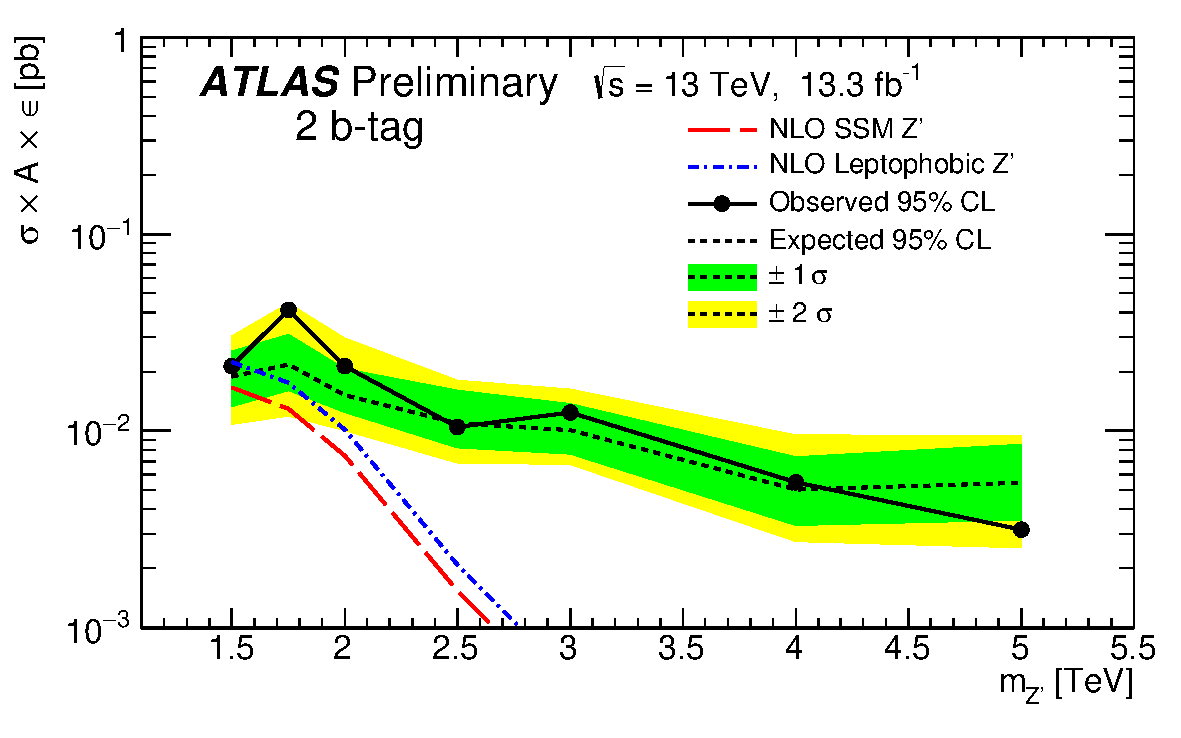
\includegraphics[width=0.9\linewidth, angle=0]{figs/Dibjet/ICHEP/lim-zprime.pdf}
   \caption[Bayesian 95\% confidence level upper limits on cross-section times acceptance times tagging efficiency
    for the $Z'$-boson using the 2 $b$-tag category.
    The observed limit the observed limit is shown by the solid black line,
    the expected limit is shown by the dotted black line
    and the 1 and 2 $\sigma$ error bands are shown by the green and yellow bands respectively.
    The theoretical predicition of $\sigma\,\text{x}\,\mathit{A}\,\text{x}\,\epsilon$
    for the Sequential Standard Model (SSM) and leptophobic $Z'$-boson are overlaid.]
           {Bayesian 95\% confidence level upper limits on cross-section times acceptance times tagging efficiency
    for the $Z'$-boson using the 2 $b$-tag category.
    The observed limit the observed limit is shown by the solid black line,
    the expected limit is shown by the dotted black line
    and the 1 and 2 $\sigma$ error bands are shown by the green and yellow bands respectively.
    The theoretical predicition of $\sigma\,\text{x}\,\mathit{A}\,\text{x}\,\epsilon$
    for the Sequential Standard Model (SSM) and leptophobic $Z'$-boson are overlaid~\cite{dibjet-ichep_conf}.
  }
  \label{fig:lim-summer_zprime}
  \vspace{1cm}
  \centering
   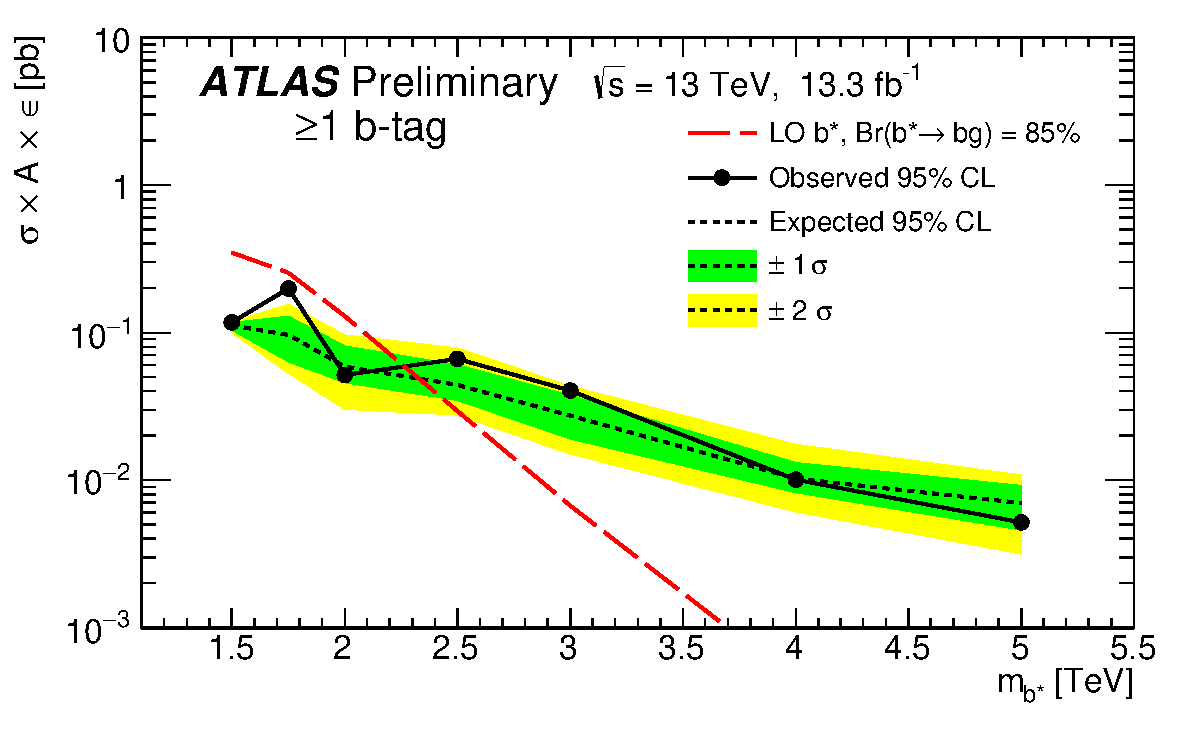
\includegraphics[width=0.9\linewidth, angle=0]{figs/Dibjet/ICHEP/lim-bstar.pdf}
   \caption[Bayesian 95\% confidence level upper limits on cross-section times acceptance times tagging efficiency
    for the $b^*$-quark using the $\geq$1 $b$-tag category.
    The observed limit the observed limit is shown by the solid black line,
    the expected limit is shown by the dotted black line
    and the 1 and 2 $\sigma$ error bands are shown by the green and yellow bands respectively.
    The theoretical predicition of $\sigma\,\text{x}\,\mathit{A}\,\text{x}\,\epsilon$
    for the $b^*$-quark is overlaid.]
           {Bayesian 95\% confidence level upper limits on cross-section times acceptance times tagging efficiency
    for the $b^*$-quark using the $\geq$1 $b$-tag category.
    The observed limit the observed limit is shown by the solid black line,
    the expected limit is shown by the dotted black line
    and the 1 and 2 $\sigma$ error bands are shown by the green and yellow bands respectively.
    The theoretical predicition of $\sigma\,\text{x}\,\mathit{A}\,\text{x}\,\epsilon$
    for the $b^*$-quark is overlaid~\cite{dibjet-ichep_conf}.
  }
  \label{fig:lim-summer_bstar}
\end{figure}

\FloatBarrier

\section{Limits: 2016\_Full}
\label{sec:lim-full}
